\documentclass[11pt]{article} 
\usepackage[english]{babel}
\usepackage[utf8]{inputenc}
\usepackage[margin=0.5in]{geometry}
\usepackage{amsmath}
\usepackage{amsthm}
\usepackage{amsfonts}
\usepackage{amssymb}
\usepackage[usenames,dvipsnames]{xcolor}
\usepackage{graphicx}
\usepackage[siunitx]{circuitikz}
\usepackage{tikz}
\usepackage[colorinlistoftodos, color=orange!50]{todonotes}
\usepackage{hyperref}
\usepackage[numbers, square]{natbib}
\usepackage{fancybox}
\usepackage{epsfig}
\usepackage{soul}
\usepackage[framemethod=tikz]{mdframed}
\usepackage[shortlabels]{enumitem}
\usepackage[version=4]{mhchem}
\usepackage{multicol}

\usepackage{mathtools}
\usepackage{comment}
\usepackage{enumitem}
\usepackage[utf8]{inputenc}
\usepackage[linesnumbered,ruled,vlined]{algorithm2e}
\usepackage{listings}
\usepackage{color}
\usepackage[numbers]{natbib}
\usepackage{subfiles}
\usepackage{tkz-berge}


\newtheorem{prop}{Proposition}[section]
\newtheorem{thm}{Theorem}[section]
\newtheorem{lemma}{Lemma}[section]
\newtheorem{cor}{Corollary}[prop]

\theoremstyle{definition}
\newtheorem{definition}{Definition}

\theoremstyle{definition}
\newtheorem{required}{Problem}

\theoremstyle{definition}
\newtheorem{ex}{Example}

\tikzset{
    vertex/.style={circle,draw,minimum size=16,inner sep=0pt,font=\normalsize},
    edgelabel/.style={rectangle,draw=none,font=\footnotesize,outer sep=0pt},
    every node/.style={vertex},
    every edge quotes/.append style={edgelabel},
    every to/.append style={every node/.style={edgelabel}},
    wide/.style={line width=4pt},
    directed/.style={arrows={-Stealth[length=7pt]},font=\small},
    }


\setlength{\marginparwidth}{3.4cm}
%#########################################################

%To use symbols for footnotes
\renewcommand*{\thefootnote}{\fnsymbol{footnote}}
%To change footnotes back to numbers uncomment the following line
%\renewcommand*{\thefootnote}{\arabic{footnote}}

% Enable this command to adjust line spacing for inline math equations.
% \everymath{\displaystyle}

% _______ _____ _______ _      ______ 
%|__   __|_   _|__   __| |    |  ____|
%   | |    | |    | |  | |    | |__   
%   | |    | |    | |  | |    |  __|  
%   | |   _| |_   | |  | |____| |____ 
%   |_|  |_____|  |_|  |______|______|
%%%%%%%%%%%%%%%%%%%%%%%%%%%%%%%%%%%%%%%

\title{
\normalfont \normalsize 
\textsc{CSCI 3104 Fall 2021 \\ 
Instructors: Profs. Grochow and Waggoner} \\
[10pt] 
\rule{\linewidth}{0.5pt} \\[6pt] 
\huge Quiz- Standard 11 \\
\rule{\linewidth}{2pt}  \\[10pt]
}
%\author{Your Name}
\date{}

\begin{document}
\definecolor {processblue}{cmyk}{0.96,0,0,0}
\definecolor{processred}{rgb}{200, 0, 0}
\definecolor{processgreen}{rgb}{0, 255, 0}
\DeclareGraphicsExtensions{.png}
\DeclareGraphicsExtensions{.gif}
\DeclareGraphicsExtensions{.jpg}

\maketitle


%%%%%%%%%%%%%%%%%%%%%%%%%
%%%%%%%%%%%%%%%%%%%%%%%%%%
%%%%%%%%%%FILL IN YOUR NAME%%%%%%%
%%%%%%%%%%AND STUDENT ID%%%%%%%%
%%%%%%%%%%%%%%%%%%%%%%%%%%
\noindent
Due Date \dotfill October / $11{th}$ / 2021 \\
Name \dotfill \textbf{Michael Ghattas} \\
Student ID \dotfill \textbf{109200649} \\


\tableofcontents

\section{Instructions}
 \begin{itemize}
	\item The solutions \textbf{should be typed}, using proper mathematical notation. We cannot accept hand-written solutions. \href{http://ece.uprm.edu/~caceros/latex/introduction.pdf}{Here's a short intro to \LaTeX.}
	\item You should submit your work through the \textbf{class Canvas page} only. Please submit one PDF file, compiled using this \LaTeX \ template.
	\item You may not need a full page for your solutions; pagebreaks are there to help Gradescope automatically find where each problem is. Even if you do not attempt every problem, please submit this document with no fewer pages than the blank template (or Gradescope has issues with it).

	\item You \textbf{may not collaborate with other students}. \textbf{Copying from any source is an Honor Code violation. Furthermore, all submissions must be in your own words and reflect your understanding of the material.} If there is any confusion about this policy, it is your responsibility to clarify before the due date. 

	\item Posting to \textbf{any} service including, but not limited to Chegg, Discord, Reddit, StackExchange, etc., for help on an assignment is a violation of the Honor Code.

	\item You \textbf{must} virtually sign the Honor Code (see Section \ref{HonorCode}). Failure to do so will result in your assignment not being graded.
\end{itemize}


\section{Honor Code (Make Sure to Virtually Sign)} \label{HonorCode}

\begin{required}
\noindent 
\begin{itemize}
\item My submission is in my own words and reflects my understanding of the material.
\item I have not collaborated with any other person.
\item I have not posted to external services including, but not limited to Chegg, Discord, Reddit, StackExchange, etc.
\item I have neither copied nor provided others solutions they can copy.
\end{itemize}

%\noindent In the specified region below, clearly indicate that you have upheld the Honor Code. Then type your name. 
\end{required}

\begin{proof}[I agree to the above, Michael Ghattas.]
%% Typing "I agree to the above," followed by your name is sufficient.
\end{proof}


\newpage
\section{Standard 11- Network Flows: Reductions}

\begin{required} \label{Problem2}
We say that two $i \rightsquigarrow j$ paths are \textit{edge-disjoint} if they do not share any common edges. Note however, these paths can (and in fact, often do) share common vertices (aside from $i$ and $j$). As an example, consider the following graph. 
\begin{itemize}
\item Observe that $0 \to 1 \to 3 \to 5 \to 6$ and $0 \to 2 \to 3 \to 6$ are edge-disjoint paths, as they do not share any directed edges. It is fine that they share the common vertex $3$.

\item Note however that $0 \to 2 \to 4 \to 6$ and $0 \to 2 \to 3 \to 6$ are \textbf{not} edge-disjoint paths, as they both share the $(0, 2)$ edge.
\end{itemize}

\begin{center}
	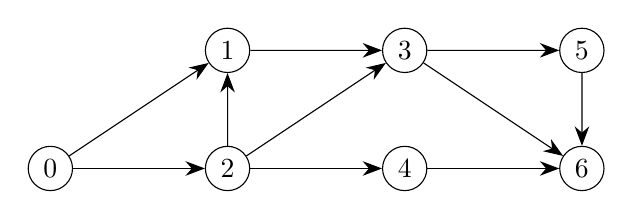
\begin{tikzpicture}[xscale=2.25,yscale=1.5]
		\node (a) at (0,0) {$0$};
		\node (b) at (1,1) {$1$};
		\node (c) at (1,0) {$2$};
		\node (d) at (2,1) {$3$};
		\node (e) at (2,0) {$4$};
        \node (f) at (3,1) {$5$};
        \node (g) at (3,0) {$6$};
	
		\draw[directed] (a) to (b);
        \draw[directed] (a) to (c);
        \draw[directed] (b) to (d);
        \draw[directed] (c) to (b);
        \draw[directed] (c) to (d);
        \draw[directed] (c) to (e);
        \draw[directed] (d) to (f);
        \draw[directed] (d) to (g);
        \draw[directed] (e) to (g);
        \draw[directed] (f) to (g);
    \end{tikzpicture}
\end{center}

\noindent Consider the following problem.
\begin{itemize}
\item \textsf{Input:} A directed graph $G(V, E)$, as well as a start node $i$ and an end node $j$. 
\item \textsf{Solution:} We seek to find a set $\mathcal{P}$ of $i \to j$ paths such that any two distinct paths $P_{1}, P_{2} \in \mathcal{P}$ are edge-disjoint, and $|\mathcal{P}|$ is maximum. That is, we seek to find a maximum set of edge-disjoint $i \to j$ paths.
\end{itemize}


\begin{enumerate}[(a)]
\item Describe how to reduce the above problem to the (one-source, one-sink) max-flow problem from class. Your description should be \textbf{general}, and not tied to a specific example. 

\begin{proof}[Answer:] \
\item \textbf{We start by noting that the maximum number of edge-disjoint $i \to j$ is equal to the maximum flow value. Thus our approach can be considered as follows:}

\begin{itemize}
\item Initially, assume that there are $(n)$ edge-disjoint paths $P_1 \to P_n$.
\item Set $w(e) = 1$ if the edge is traversed in any $P_i$, where $i = \{1,...,n\}$
\item Set $w(e) = 0$ if the edge is not traversed in any $P_i$, where $i = \{1,...,n\}$
\item The maximum flow formulation assigns a unit capacity to every edge
\item Given that our paths are edge-disjoint, our flow-augmenting path $f$ has a cardinality $val(f) = n$
\item The maximum number of edge-disjoint $i \to j$ paths equals maximum flow value.
\item Assume that the maximum flow value is $(n)$, then there exists $0 - 1$ flow $f$ of value $(n)$
\item Consider the $source$ node $s$, and the edge $(s, u)$ with $f(s, u) = 1$, then there should exist an edge $(u, v)$ with $f(u, v)=1$.
\item Consider the $sink$ node $t$, proceed while continuously choosing a new edge along the chosen path $P_i$ until reaching $t$
\item Finally, repeating this process until there are no more edge-disjoint paths should produces $(n)$ edge-disjoint paths
\end{itemize}
%Your answer here.
\end{proof}


\item Using your reduction, find a maximum set of edge-disjoint paths from $0 \rightsquigarrow 6$ in the graph above. Show your work, as well as your final answer. Note that there may be multiple maximum-size sets $\mathcal{P}$ in the graph above; you need only find one such set $\mathcal{P}$ of edge-disjoint paths, as long as it has the largest number of paths possible.

\begin{proof}[Answer:] \
\item \textbf{We will utilize the approach from part $(a)$ to avoid repetition of information. Thus our chosen paths that make up $\mathcal{P}$ are:}

\begin{center}
	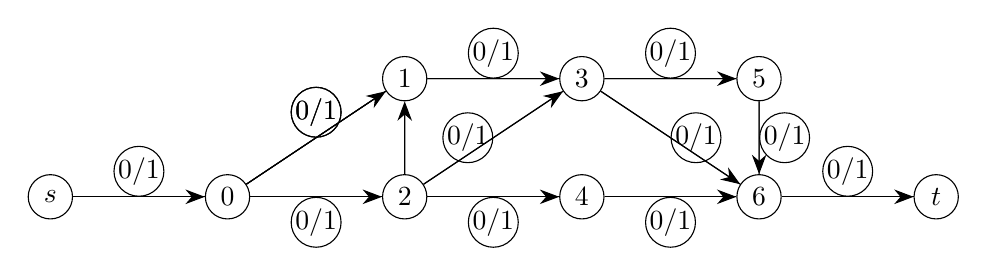
\begin{tikzpicture}[xscale=2.25,yscale=1.5]
		\node (s) at (-1,0) {$s$};
		\node (a) at (0,0) {$0$};
		\node (b) at (1,1) {$1$};
		\node (c) at (1,0) {$2$};
		\node (d) at (2,1) {$3$};
		\node (e) at (2,0) {$4$};
       		 \node (f) at (3,1) {$5$};
       		 \node (g) at (3,0) {$6$};
       		 \node (t) at (4,0) {$t$};
	
	\draw[directed] (s) to (a);
	\draw[directed] (a) to (b);
        \draw[directed] (a) to (c);
        \draw[directed] (b) to (d);
        \draw[directed] (c) to (b);
        \draw[directed] (c) to (d);
        \draw[directed] (c) to (e);
        \draw[directed] (d) to (f);
        \draw[directed] (d) to (g);
        \draw[directed] (e) to (g);
        \draw[directed] (f) to (g);
        \draw[directed] (g) to (t);
        
        	\path (a) edge node[above] {$0 / 1$} (b);
        	\path (b) edge node[above] {$0 / 1$} (d);	
        	\path (d) edge node[above] {$0 / 1$} (f);	
        	\path (f) edge node[right] {$0 / 1$} (g);	
        	\path (a) edge node[above] {$0 / 1$} (b);
	
        	\path (s) edge node[above] {$0 / 1$} (a);		
        	\path (a) edge node[below] {$0 / 1$} (c);	
        	\path (c) edge node[below] {$0 / 1$} (e);
        	\path (c) edge node[left] {$0 / 1$} (d);	
	\path (d) edge node[right] {$0 / 1$} (g);			
        	\path (e) edge node[below] {$0 / 1$} (g);
        	\path (g) edge node[above] {$0 / 1$} (t);		
    \end{tikzpicture}
\end{center}

\begin{center}
	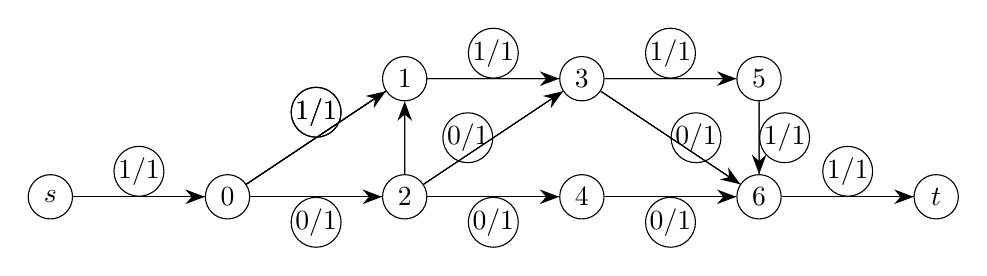
\begin{tikzpicture}[xscale=2.25,yscale=1.5]
		\node (s) at (-1,0) {$s$};
		\node (a) at (0,0) {$0$};
		\node (b) at (1,1) {$1$};
		\node (c) at (1,0) {$2$};
		\node (d) at (2,1) {$3$};
		\node (e) at (2,0) {$4$};
       		 \node (f) at (3,1) {$5$};
       		 \node (g) at (3,0) {$6$};
       		 \node (t) at (4,0) {$t$};
	
	\draw[directed] (s) to (a);
	\draw[directed] (a) to (b);
        \draw[directed] (a) to (c);
        \draw[directed] (b) to (d);
        \draw[directed] (c) to (b);
        \draw[directed] (c) to (d);
        \draw[directed] (c) to (e);
        \draw[directed] (d) to (f);
        \draw[directed] (d) to (g);
        \draw[directed] (e) to (g);
        \draw[directed] (f) to (g);
        \draw[directed] (g) to (t);
        
        	\path (s) edge node[above] {$1 / 1$} (a);	        
        	\path (a) edge node[above] {$1 / 1$} (b);
        	\path (b) edge node[above] {$1 / 1$} (d);	
        	\path (d) edge node[above] {$1 / 1$} (f);	
        	\path (f) edge node[right] {$1 / 1$} (g);	
        	\path (a) edge node[above] {$1 / 1$} (b);
        	\path (g) edge node[above] {$1 / 1$} (t);	
		
        	\path (a) edge node[below] {$0 / 1$} (c);	
        	\path (c) edge node[below] {$0 / 1$} (e);
        	\path (c) edge node[left] {$0 / 1$} (d);	
	\path (d) edge node[right] {$0 / 1$} (g);			
        	\path (e) edge node[below] {$0 / 1$} (g);	
    \end{tikzpicture}
\end{center}

\begin{center}
	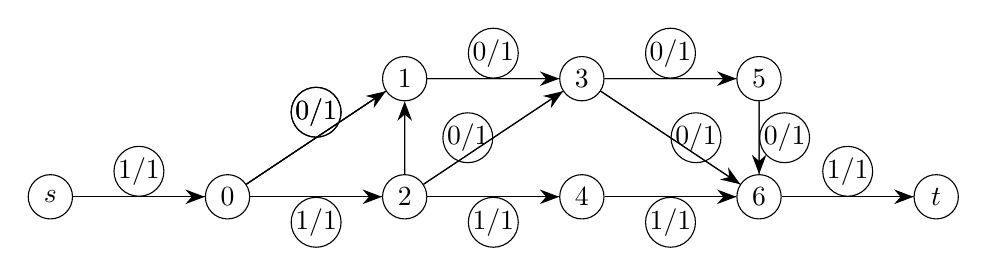
\begin{tikzpicture}[xscale=2.25,yscale=1.5]
		\node (s) at (-1,0) {$s$};
		\node (a) at (0,0) {$0$};
		\node (b) at (1,1) {$1$};
		\node (c) at (1,0) {$2$};
		\node (d) at (2,1) {$3$};
		\node (e) at (2,0) {$4$};
       		 \node (f) at (3,1) {$5$};
       		 \node (g) at (3,0) {$6$};
       		 \node (t) at (4,0) {$t$};
	
	\draw[directed] (s) to (a);
	\draw[directed] (a) to (b);
        \draw[directed] (a) to (c);
        \draw[directed] (b) to (d);
        \draw[directed] (c) to (b);
        \draw[directed] (c) to (d);
        \draw[directed] (c) to (e);
        \draw[directed] (d) to (f);
        \draw[directed] (d) to (g);
        \draw[directed] (e) to (g);
        \draw[directed] (f) to (g);
        \draw[directed] (g) to (t);
        
        	\path (a) edge node[above] {$0 / 1$} (b);
        	\path (b) edge node[above] {$0 / 1$} (d);	
        	\path (d) edge node[above] {$0 / 1$} (f);	
        	\path (f) edge node[right] {$0 / 1$} (g);	
        	\path (a) edge node[above] {$0 / 1$} (b);
	
        	\path (s) edge node[above] {$1 / 1$} (a);		
        	\path (a) edge node[below] {$1 / 1$} (c);	
        	\path (c) edge node[below] {$1 / 1$} (e);
        	\path (c) edge node[left] {$0 / 1$} (d);	
	\path (d) edge node[right] {$0 / 1$} (g);			
        	\path (e) edge node[below] {$1 / 1$} (g);
        	\path (g) edge node[above] {$1 / 1$} (t);		
    \end{tikzpicture}
\end{center}

\begin{itemize}
\item $P_1$ = $s \to 0 \to 1 \to 3 \to 5 \to 6 \to t$
\item $P_2$ = $s \to 0 \to 2 \to 4 \to 6 \to t$
\end{itemize}
\item \textbf{Since there are no more edge-disjoint possible paths available for us to choose from after choosing $P_1$ and $P_2$, $\mathcal{P}$ = $\{P_1, P_2\}$, and $|\mathcal{P}|$ = $2$, which is the maximum flow value.}

%Your answer here
\end{proof}


% Either type your answer in above, or uncomment the \includegraphics command
% and use it to insert an appropirate image. Try experimenting with the scale 
% 0.9 the width option to resize your image if necessary.

%\includegraphics[width=0.9\textwidth]{solution.jpg}

\end{enumerate}

\end{required}

%%%%%%%%%%%%%%%%%%%%%%%%%%%%%%%%%%%%%%%%%%%%%%%%%%
\end{document} % NOTHING AFTER THIS LINE IS PART OF THE DOCUMENT



